\documentclass[11pt]{article}
\usepackage[margin=0.75in]{geometry}
\usepackage{amsmath}
\usepackage{enumitem}
\usepackage{color,soul}
\usepackage{multicol}
\usepackage{tikz}

\newcommand{\ds}{\displaystyle}

\begin{document}
\newcounter{enumCount}
\pagestyle{empty}
\subsection*{Math 141 - Homework 5 \hfill Name: \underline{\hspace*{2in}}}

\textit{Find the derivative of each function.}
\begin{multicols}{3}
\begin{enumerate}
\item $f(x) = x + \sqrt{x}$
\item $y = x^4 + \dfrac{2}{x}$
\item $\ds g(x) = 2x^2\left(5x^3 + \frac{4}{x} \right)$
\setcounter{enumCount}{\theenumi}
\end{enumerate}
\end{multicols}
\vfill

\noindent
\begin{multicols}{3}
\begin{enumerate}
\setcounter{enumi}{\theenumCount}
\item $z = \dfrac{x^3 + 3x^2 - 1}{3}$
\item $h(t) = (t^2 + 5) \sin t$
\item $f(x) = \dfrac{x^2}{x^2 + 4}$
\setcounter{enumCount}{\theenumi}
\end{enumerate}
\end{multicols}
\vfill


\begin{enumerate}
\setcounter{enumi}{\theenumCount}
\item Let $f(x) = x^{3} - 9 x^{2} + 15x - 1$. 
\begin{enumerate}
\item Find all values of $x$ where the slope of the tangent line is $15$. 
\vfill
\item Find the values of $x$ where the tangent line is horizontal. 
\vfill
\end{enumerate}

\item Find an equation for the tangent line to the function $y = x^2 - 5x + 2$ at the point $(6,8)$.
\vfill


\newpage
\item Suppose that a particle moves with position $s(t) = t^{3} - 9 t^{2} + 24 t$.
\begin{enumerate}
\item Find formulas for the velocity $v(t)$ and acceleration $a(t)$ of the particle. \vfill
\item Find the time intervals where the velocity of the particle is positive.
\end{enumerate}
\vfill

\item Let $h(x) = f(x) g(x)$ where $f$ and $g$ are shown in the graph below.  Find the values of the following derivatives.

\begin{center}
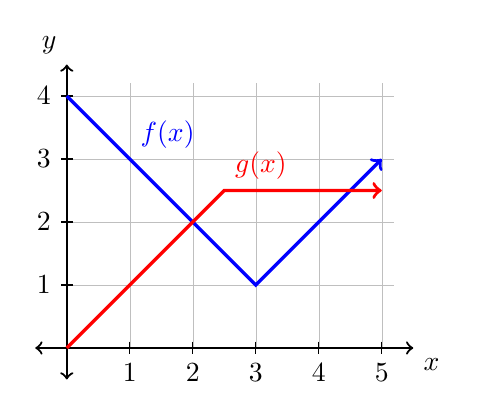
\begin{tikzpicture}[xscale=0.8,yscale=0.8]
\draw[very thin,gray!50] (0,0) grid (5.2,4.2);
\draw[thick,<->] (-0.5,0) -- (5.5,0) node[below right] {$x$};
\draw[thick,<->] (0,-0.5) -- (0,4.5) node[above left] {$y$};
\foreach \x in {1,2,3,4,5} {
  \draw (\x,0.1) -- (\x,-0.1) node[below] {\x};
}
\foreach \y in {4,3,2,1} {
  \draw (0.1,\y) -- (-0.1,\y) node[left] {\y};
}
\draw[very thick, blue, ->] (0,4) -- (1,3) node[above right] {$f(x)$} -- (3,1) -- (5,3);
\draw[very thick, red, ->] (0,0) -- (2.5,2.5) node[above right] {$g(x)$} -- (5,2.5);
\end{tikzpicture}
\end{center}
\begin{enumerate}
\item $h'(1)$ 
\bigskip
\item $h'(4)$ 
\bigskip
\end{enumerate}

\item A rock is tossed upwards with initial velocity 28 feet per second by a person standing on a building 60 feet above the ground.  The height of the rock is $h(t) = -16t^2 + 28t + 60$. 
\begin{enumerate}
\item What is the acceleration of gravity in this problem? 
\vfill

\item What is the velocity of the rock when it hits the ground at time $t = 3$ seconds?
\end{enumerate}
\vfill


\setcounter{enumCount}{\theenumi}
\end{enumerate}

\end{document}
